    \tikzset{mnode/.style = {shape = circle,
                                    color = black,
                                    inner sep=1pt,
                                    minimum size = 4 pt,
                                    font=\scriptsize\sffamily,
                                    draw}}
\begin{tabular}{|c|c||c|c|c|c|}
	\hline
	\multicolumn{2}{|c||}{$n=2$} 
	& \multicolumn{4}{c|}{$n=3$} \\
	\begin{tikzpicture}[mnode/.style = {shape = circle,
                                    color = black,
                                    inner sep=1pt,
                                    minimum size = 4 pt,
                                    font=\scriptsize\sffamily,
                                    draw}]
		\node[mnode] (1) at (0,0) {};
		\node[mnode] (2) at (1,0) {};
	\end{tikzpicture}
	& 
	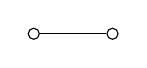
\begin{tikzpicture}[mnode/.style = {shape = circle,
                                    color = black,
                                    inner sep=1pt,
                                    minimum size = 4 pt,
                                    font=\scriptsize\sffamily,
                                    draw}]
		\node[mnode] (1) at (0,0) {};
		\node[mnode] (2) at (1,0) {};
		\path (1) edge (2);
	\end{tikzpicture}
	& 
	\begin{tikzpicture}[mnode/.style = {shape = circle,
                                    color = black,
                                    inner sep=1pt,
                                    minimum size = 4 pt,
                                    font=\scriptsize\sffamily,
                                    draw}]
		\node[mnode] (1) at (0,0) {};
		\node[mnode] (2) at (1,0) {};
		\node[mnode] (3) at (60:1) {};
	\end{tikzpicture}
	& 
	\begin{tikzpicture}[mnode/.style = {shape = circle,
                                    color = black,
                                    inner sep=1pt,
                                    minimum size = 4 pt,
                                    font=\scriptsize\sffamily,
                                    draw}]
		\node[mnode] (1) at (0,0) {};
		\node[mnode] (2) at (1,0) {};
		\node[mnode] (3) at (60:1) {};
		\path (1) edge (2);
	\end{tikzpicture}
	& 
	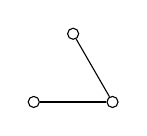
\begin{tikzpicture}[mnode/.style = {shape = circle,
                                    color = black,
                                    inner sep=1pt,
                                    minimum size = 4 pt,
                                    font=\scriptsize\sffamily,
                                    draw}]
		\node[mnode] (1) at (0,0) {};
		\node[mnode] (2) at (1,0) {};
		\node[mnode] (3) at (60:1) {};
		\path (1) edge (2);
		\path (2) edge (3);
	\end{tikzpicture}
	& 
	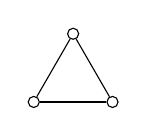
\begin{tikzpicture}[mnode/.style = {shape = circle,
                                    color = black,
                                    inner sep=1pt,
                                    minimum size = 4 pt,
                                    font=\scriptsize\sffamily,
                                    draw}]
		\node[mnode] (1) at (0,0) {};
		\node[mnode] (2) at (1,0) {};
		\node[mnode] (3) at (60:1) {};
		\path (1) edge (2);
		\path (2) edge (3);
		\path (3) edge (1);
	\end{tikzpicture}
	\\
	\hline
\end{tabular}

\begin{tabular}{|c|c|c|c|c|c|c|}
	\hline
	\multicolumn{7}{|c|}{$n=4$} \\
	\begin{tikzpicture}[mnode/.style = {shape = circle,
                                    color = black,
                                    inner sep=1pt,
                                    minimum size = 4 pt,
                                    font=\scriptsize\sffamily,
                                    draw}]
		\node[mnode] (1) at (0,0) {};
		\node[mnode] (2) at (1,0) {};
		\node[mnode] (3) at (1,1) {};
		\node[mnode] (4) at (0,1) {};
	\end{tikzpicture}
	& 
	\begin{tikzpicture}[mnode/.style = {shape = circle,
                                    color = black,
                                    inner sep=1pt,
                                    minimum size = 4 pt,
                                    font=\scriptsize\sffamily,
                                    draw}]
		\node[mnode] (1) at (0,0) {};
		\node[mnode] (2) at (1,0) {};
		\node[mnode] (3) at (1,1) {};
		\node[mnode] (4) at (0,1) {};
		\path (1) edge (2);
	\end{tikzpicture}
	& 
	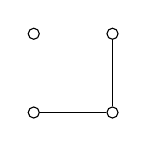
\begin{tikzpicture}[mnode/.style = {shape = circle,
                                    color = black,
                                    inner sep=1pt,
                                    minimum size = 4 pt,
                                    font=\scriptsize\sffamily,
                                    draw}]
		\node[mnode] (1) at (0,0) {};
		\node[mnode] (2) at (1,0) {};
		\node[mnode] (3) at (1,1) {};
		\node[mnode] (4) at (0,1) {};
		\path (1) edge (2);
		\path (2) edge (3);
	\end{tikzpicture}
	& 
	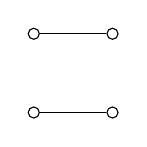
\begin{tikzpicture}[mnode/.style = {shape = circle,
                                    color = black,
                                    inner sep=1pt,
                                    minimum size = 4 pt,
                                    font=\scriptsize\sffamily,
                                    draw}]
		\node[mnode] (1) at (0,0) {};
		\node[mnode] (2) at (1,0) {};
		\node[mnode] (3) at (1,1) {};
		\node[mnode] (4) at (0,1) {};
		\path (1) edge (2);
		\path (3) edge (4);
	\end{tikzpicture}
	& 
	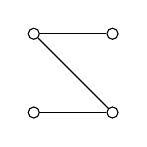
\begin{tikzpicture}[mnode/.style = {shape = circle,
                                    color = black,
                                    inner sep=1pt,
                                    minimum size = 4 pt,
                                    font=\scriptsize\sffamily,
                                    draw}]
		\node[mnode] (1) at (0,0) {};
		\node[mnode] (2) at (1,0) {};
		\node[mnode] (3) at (1,1) {};
		\node[mnode] (4) at (0,1) {};
		\path (1) edge (2);
		\path (2) edge (4);
		\path (4) edge (3);
	\end{tikzpicture}
	&
	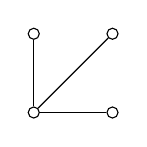
\begin{tikzpicture}[mnode/.style = {shape = circle,
                                    color = black,
                                    inner sep=1pt,
                                    minimum size = 4 pt,
                                    font=\scriptsize\sffamily,
                                    draw}]
		\node[mnode] (1) at (0,0) {};
		\node[mnode] (2) at (1,0) {};
		\node[mnode] (3) at (1,1) {};
		\node[mnode] (4) at (0,1) {};
		\path (1) edge (2);
		\path (1) edge (3);
		\path (1) edge (4);
	\end{tikzpicture}
	& 
	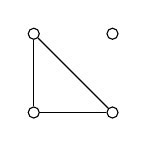
\begin{tikzpicture}[mnode/.style = {shape = circle,
                                    color = black,
                                    inner sep=1pt,
                                    minimum size = 4 pt,
                                    font=\scriptsize\sffamily,
                                    draw}]
		\node[mnode] (1) at (0,0) {};
		\node[mnode] (2) at (1,0) {};
		\node[mnode] (3) at (1,1) {};
		\node[mnode] (4) at (0,1) {};
		\path (1) edge (2);
		\path (1) edge (4);
		\path (2) edge (4);
	\end{tikzpicture} 
	\\
	\hline
	\multicolumn{7}{|c|}{ } \\
	 & 
	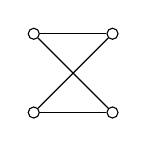
\begin{tikzpicture}[mnode/.style = {shape = circle,
                                    color = black,
                                    inner sep=1pt,
                                    minimum size = 4 pt,
                                    font=\scriptsize\sffamily,
                                    draw}]
		\node[mnode] (1) at (0,0) {};
		\node[mnode] (2) at (1,0) {};
		\node[mnode] (3) at (1,1) {};
		\node[mnode] (4) at (0,1) {};
		\path (1) edge (2);
		\path (3) edge (4);
		\path (1) edge (3);
		\path (2) edge (4);
	\end{tikzpicture}
	& 
	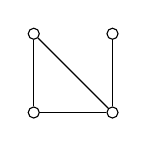
\begin{tikzpicture}[mnode/.style = {shape = circle,
                                    color = black,
                                    inner sep=1pt,
                                    minimum size = 4 pt,
                                    font=\scriptsize\sffamily,
                                    draw}]
		\node[mnode] (1) at (0,0) {};
		\node[mnode] (2) at (1,0) {};
		\node[mnode] (3) at (1,1) {};
		\node[mnode] (4) at (0,1) {};
		\path (1) edge (2);
		\path (1) edge (4);
		\path (2) edge (4);
		\path (2) edge (3);
	\end{tikzpicture}
	& 
	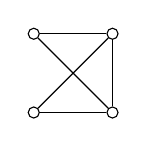
\begin{tikzpicture}[mnode/.style = {shape = circle,
                                    color = black,
                                    inner sep=1pt,
                                    minimum size = 4 pt,
                                    font=\scriptsize\sffamily,
                                    draw}]
		\node[mnode] (1) at (0,0) {};
		\node[mnode] (2) at (1,0) {};
		\node[mnode] (3) at (1,1) {};
		\node[mnode] (4) at (0,1) {};
		\path (1) edge (2);
		\path (3) edge (4);
		\path (1) edge (3);
		\path (2) edge (4);
		\path (2) edge (3);
	\end{tikzpicture}
	& 
	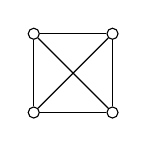
\begin{tikzpicture}[mnode/.style = {shape = circle,
                                    color = black,
                                    inner sep=1pt,
                                    minimum size = 4 pt,
                                    font=\scriptsize\sffamily,
                                    draw}]
		\node[mnode] (1) at (0,0) {};
		\node[mnode] (2) at (1,0) {};
		\node[mnode] (3) at (1,1) {};
		\node[mnode] (4) at (0,1) {};
		\path (1) edge (2);
		\path (3) edge (4);
		\path (1) edge (3);
		\path (2) edge (4);
		\path (2) edge (3);
		\path (1) edge (4);
	\end{tikzpicture}
	& 
	& 
	\\
	\hline
\end{tabular}